%coupling_shifting

In this section we consider shifting the waveguide to affect the light properties in second propagating track. As a 3D model the waveguide can be shifted on transverse and or longitude directions as Fig. \ref{fig:shift_all_axis}.
\begin{figure}[!ht]
\centering
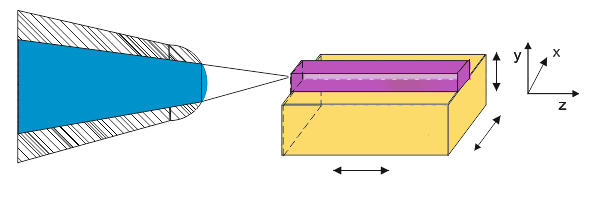
\includegraphics[width=0.7\textwidth]{bilder/shift_all_axis}
\caption{Displacing the waveguide along X, Y, Z-Axis.}
\label{fig:shift_all_axis}
\end{figure}

\begin{itemize}
\item Shift the waveguide along X-Axis: Relocate the waveguide from $-0.5\mu$m to $0.5\mu$m:
%\begin{figure}[!ht]
%\centering
%%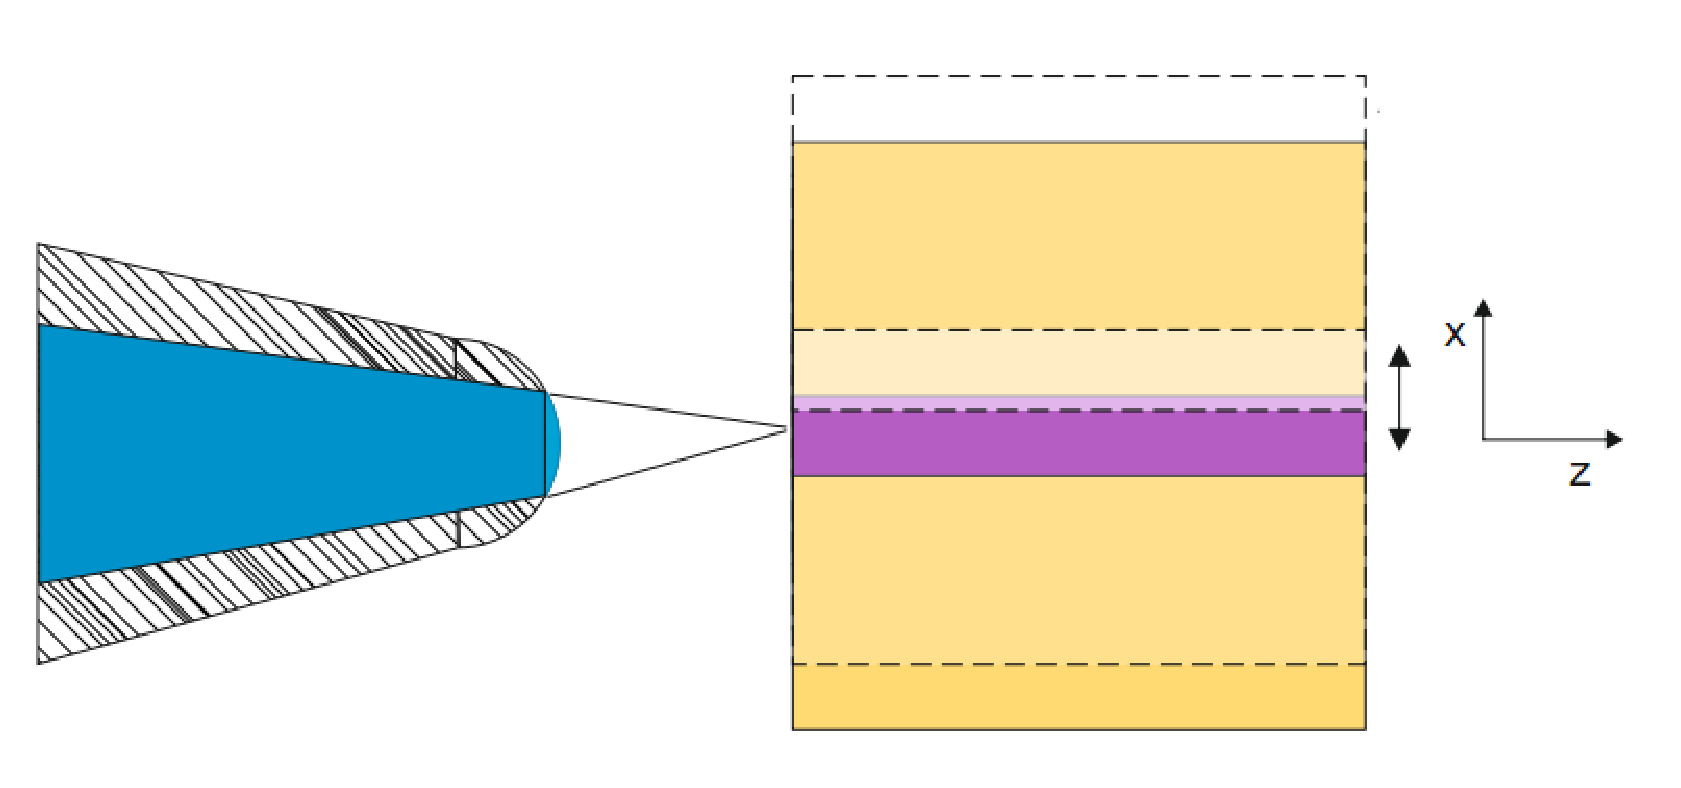
\includegraphics[width=0.7\textwidth]{bilder/shift_x_axis}
%%\caption{Displacing the waveguide along x-axis.}
%\label{fig:shift_x_axis}
%\end{figure}
\item Shift the waveguide along Y-Axis: Relocate the waveguide from $-0.5\mu$m to $0.5\mu$m:
%\begin{figure}[!ht]
%\centering
%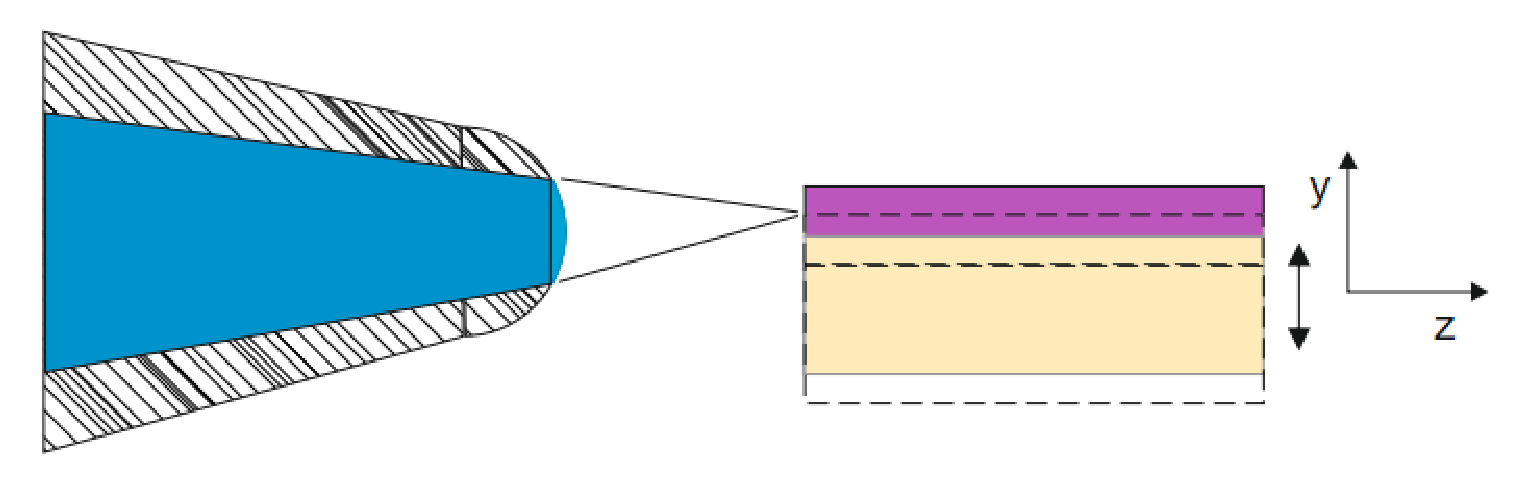
\includegraphics[width=0.7\textwidth]{bilder/shift_y_axis}
%\caption{Displacing the waveguide along y-axis.}
%\label{fig:shift_y_axis}
%\end{figure}
\item Shift the waveguide along Z-Axis: Relocate the waveguide from $-0.5\mu$m to $0.5\mu$m:
%\begin{figure}[!ht]
%\centering
%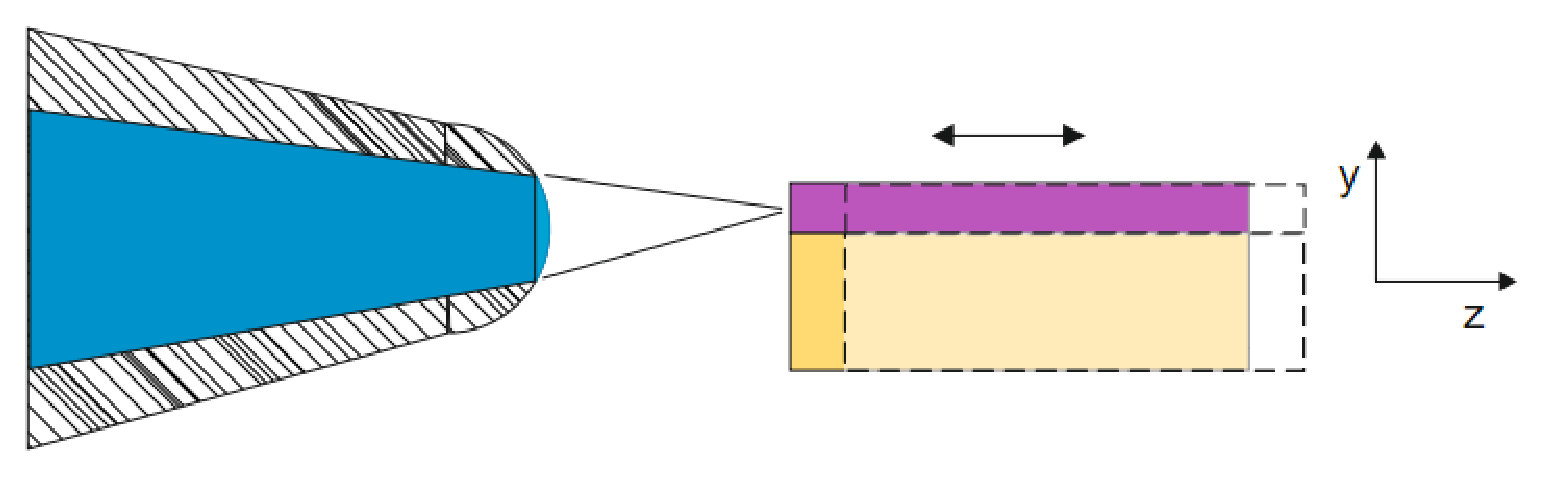
\includegraphics[width=0.7\textwidth]{bilder/shift_z_axis}
%\caption{Displacing the waveguide along z-axis.}
%\label{fig:shift_z_axis}
%\end{figure}
\end{itemize}
Performe above arrangements and record their simulation results $|S_{21}|$ in Tab. \ref{tab:shift_result}:\\

\begin{table}[!ht]
\caption{Coupling efficiency by shifting the waveguide along X,Y and Z-Axis.}
\centering
\begin{tabular}{c|ccc}
\hline
Shift distance & X-Axis & Y-Axis & Z-Axis \\
\hline
$-0.5\mu$m 		&$32.4\%$	&$32.4\%$&$46.6\%$	\\
$-0.4\mu$m		&$37.3\%$	&$36.5\%$&$47\%$	\\
$-0.3\mu$m 		&$41.9\%$	&$41.3\%$&$48.2\%$	\\
$-0.2\mu$m	  &$45.5\%$	&$45.2\%$&$49.1\%$	\\
$-0.1\mu$m		&$48\%$	&$47.8\%$&$49.1\%$	\\
$0\mu$m			  &$48.9\%$	&$48.9\%$&$48.9\%$	\\
$0.1\mu$m			&$47.8\%$	&$48.4\%$&$48.9\%$	\\
$0.2\mu$m			&$45.5\%$	&$46.4\%$&$49.4\%$	\\
$0.3\mu$m			&$41.9\%$	&$42.9\%$&$49.7\%$	\\
$0.4\mu$m			&$37.5\%$	&$38.5\%$&$49.5\%$	\\
$0.5\mu$m			&$32.3\%$	&$33.1\%$&$48.8\%$	\\
\hline
\end{tabular}
\label{tab:shift_result}
\end{table}
According results in the table we can draw curves in Fig. \ref{fig:shift_curve}, which presents coupling efficiencies due to waveguide shifting. For transversal shifting among range $-0.5\mu$m to $0.5\mu$m the coupling efficiency falls very quickly in vertical or horizontal directions from $48.9\%$ to about $32\%$.  In another word, the coupling efficiency stands for the highest value of $48.9\%$ when there is not shifting in transversal directions. From this Figure it can also be revealed that coupling efficiencies are symmetric due to positive and negative X-Axis shifting. While the coupling efficiencies due to negative and positive Y-Axis shifting are not symmetric. This trend can be explained by the geometric characteristic of the waveguide, which is same in X-Dimension and different in Y-Dimension.  In longitudinal direction among the shifting range $-0.5\mu$m to $0.5\mu$m the lowest coupling efficiency is $46\%$ at distance $3.5\mu$m from TLF, while the highest coupling efficiency of $49.7\%$ due to shifting along Z-Axis stands not at working distance $4\mu$m but $4.3\mu$m, which agree with the estimation of minimum spot location about $4.26\mu$m at section \ref{sect:model_model_model_TLF}. \\

\begin{figure}[!ht]
\centering
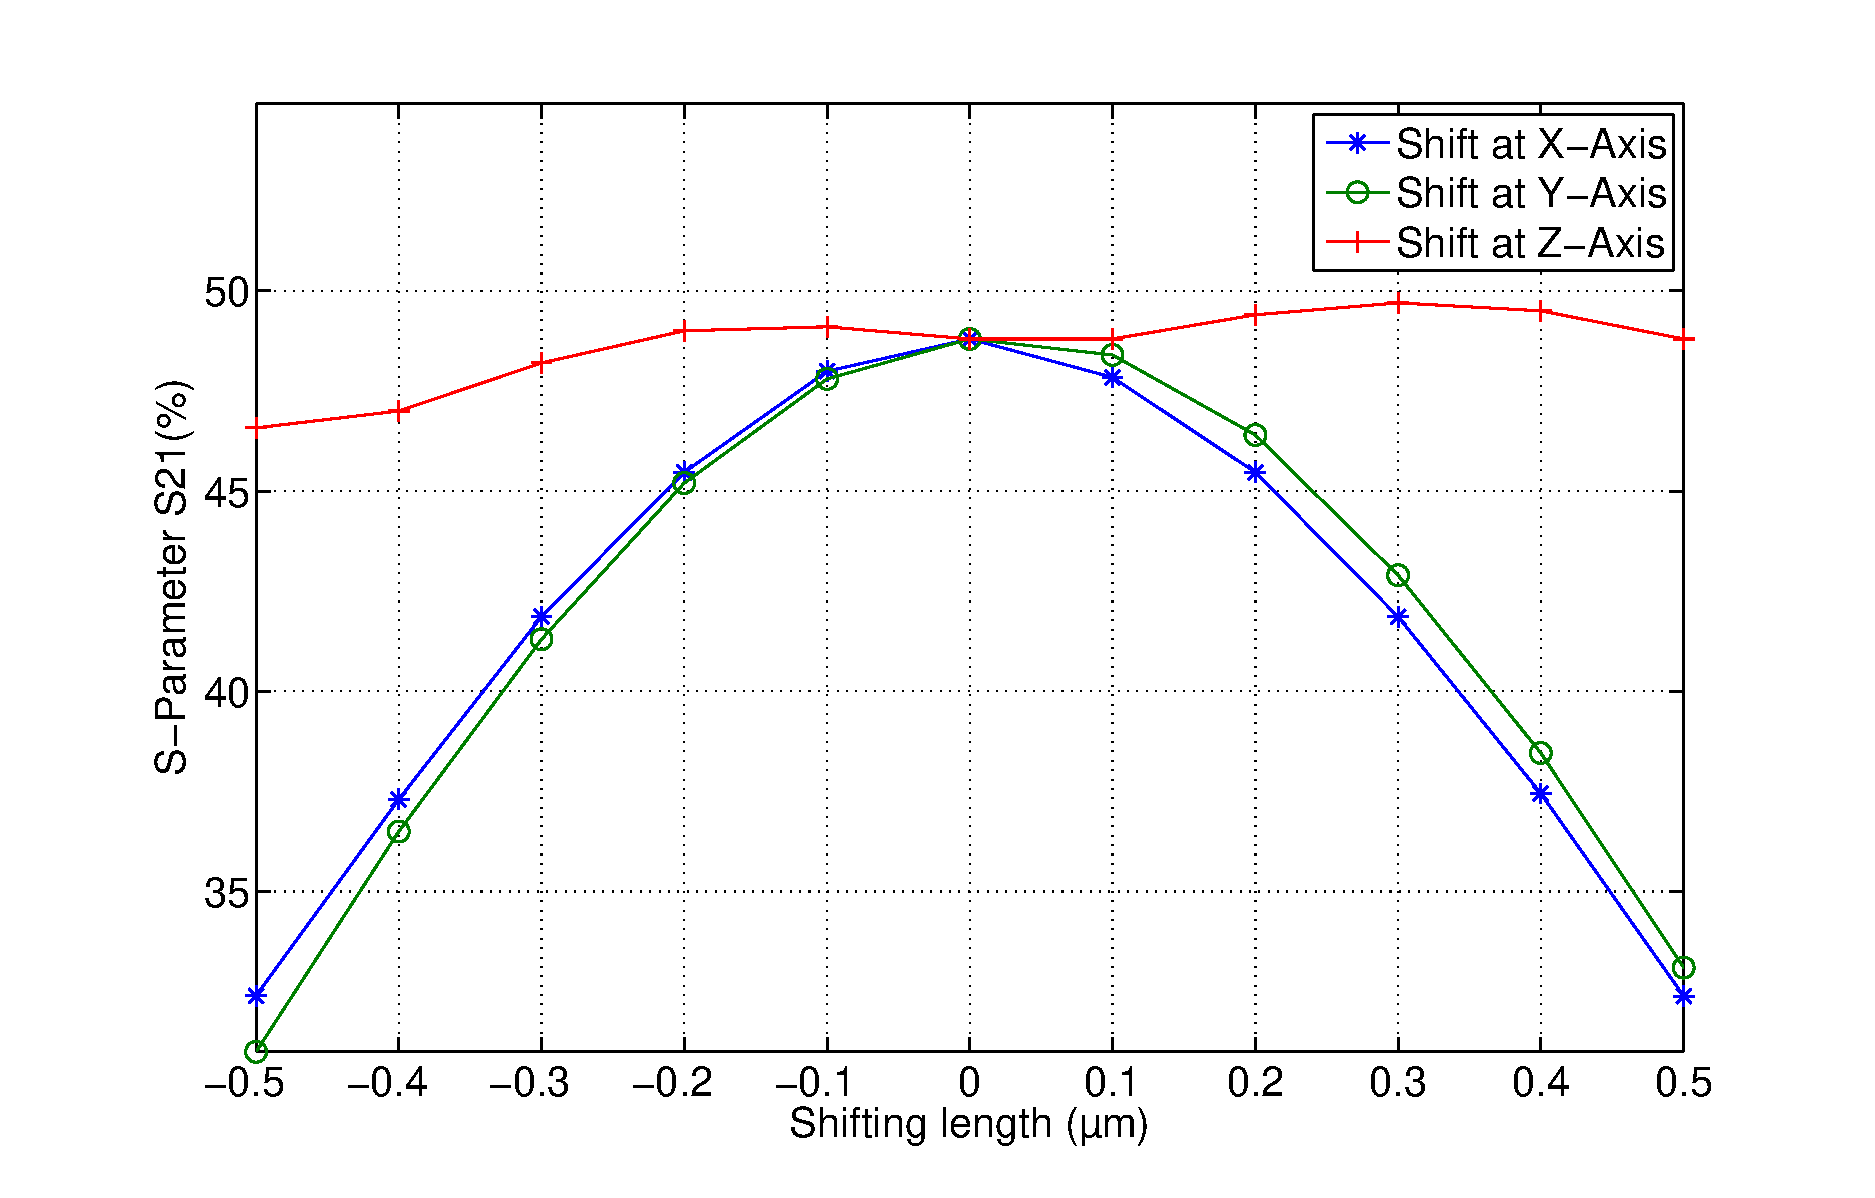
\includegraphics[width=0.8\textwidth]{bilder/shift_curve}
\caption{Coupling efficiency due to the displacement of the wavguide.}
\label{fig:shift_curve}
\end{figure}

Through above discussions following can be concluded:
\begin{itemize} 
\item Shifting in transversal directions cannot improve the coupling efficiency and obviously affect the coupling ability. 
\item Shifting in longitudinal direction can gently affect the coupling ability. 
\end{itemize}
Although the location the minimum spot lies not on the working distance $4\mu$m, displacement of the waveguide cannot obviously improve the coupling efficiency, difference of $1\%$. Hereby the working distance will be maintained in following simulations.\\
